\documentclass[a4paper,10pt]{article}
\usepackage[margin=1in]{geometry}
\usepackage{amsmath,amsthm,amssymb,amsfonts,stmaryrd}
\usepackage{soul}
\usepackage{array}
\usepackage{empheq}
\usepackage{xfrac}
\usepackage{minibox}
\usepackage{enumitem}
	\setlist{nosep} % or \setlist{noitemsep} to leave space around whole list
\usepackage{color}
\usepackage{blkarray}
\setcounter{MaxMatrixCols}{20}
\usepackage{showlabels}
\usepackage{arydshln}	% Dotted lines in arrays
\usepackage{adjustbox}
\usepackage{hyperref}
\hypersetup{
  colorlinks   = true, %Colours links instead of ugly boxes
  urlcolor     = blue, %Colour for external hyperlinks
  linkcolor    = blue, %Colour of internal links
  citecolor   = red %Colour of citations
}
\usepackage{cleveref}


\newtheorem{lemma}{Lemma}
\newtheorem{definition}{Definition}
\newtheorem{theorem}{Theorem}
\newtheorem{corollary}{Corollary}

\newcommand{\tcb}{\textcolor{blue}}
\newcommand{\todo}[1]{\textcolor{red}{[TODO\@: #1]}}


\begin{document}
\allowdisplaybreaks

% ---------------------------------------------------------------------------------------------- %
% ---------------------------------------------------------------------------------------------- %
% ---------------------------------------------------------------------------------------------- %
\section{Tom}

Let $\eta,\beta > 0$ be real constants and $\mathcal{L}$ a spatial operator with
negative field of values, $W(\mathcal{L} \leq 0$. Now suppose we want to precondition
the quadratic polynomial in $\mathcal{L}$,
%
\begin{align*}
Q := (\eta I - \mathcal{L})^2 + \beta^2 I.
\end{align*}
%
I derived some nice field of values analysis that shows using
%
\begin{align*}
P_\eta := (\eta I - \mathcal{L})^{-2}
\end{align*}
%
results in a nicely bounded field of values show below:
%
\begin{figure}[h!]
\centering
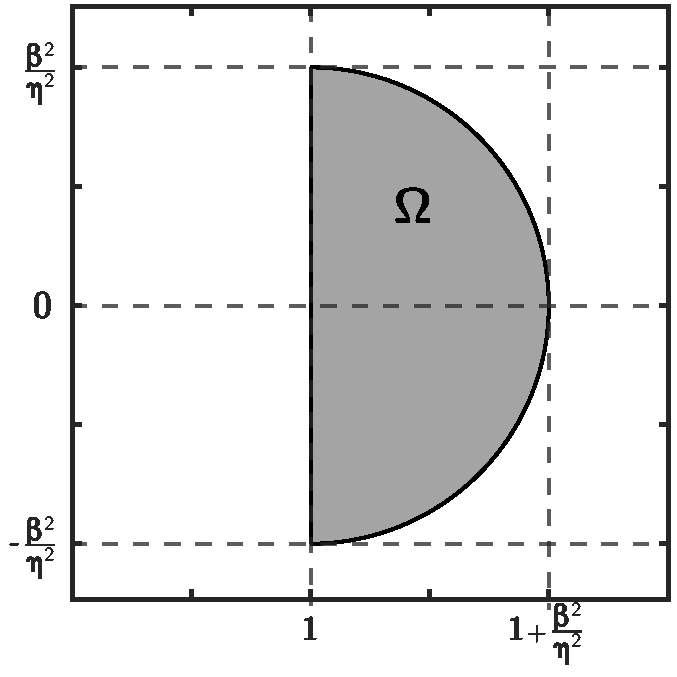
\includegraphics[width = 0.3\textwidth]{./fov_fig.pdf}
\caption{}
\label{fig:bound}
\end{figure}
%

However, $\eta$ is probably not the best constant to use. For SPD matrices, 
somebody proved that using a constant $k := \sqrt{\eta^2+\beta^2}$ and
preconditioner
%
\begin{align*}
P_k := (k I - \mathcal{L})^{-2}
\end{align*}
%
is a much better choice for $\beta \gg \eta$. I am trying to figure out if
anything similar can be said for the FOV (or other more general types of
analysis/operator).

Note that for real $k>0$, $W\left[\left(I - \tfrac{1}{k}\mathcal{L}\right)^{-1}\right]$ and
$W\left[\left(I - \tfrac{1}{k}\mathcal{L}\right)^{-2}\right]$ are contained in
the positive half unit circle. Now consider the more general preconditioning
%
\begin{align}\nonumber
(kI - \mathcal{L})^{-2}\Big[(nI - \mathcal{L})^2 + \beta^2 I\Big] 
	& = (kI - \mathcal{L})^{-2}\Big[(\eta-k)I + (kI - \mathcal{L}))^2 + \beta^2 I\Big] \\
& = (kI - \mathcal{L})^{-2}\Big[(k-\eta)^2I - 2(k-\eta)(kI - \mathcal{L}) + (kI - \mathcal{L})^2 + \beta^2 I\Big] \nonumber\\
& = I - 2(k-\eta)(kI - \mathcal{L})^{-1} + (\beta^2 + (k-\eta)^2)(kI - \mathcal{L})^{-2} \nonumber\\
& = I - 2\frac{k-\eta}{k}\left(I - \tfrac{1}{k}\mathcal{L}\right)^{-1} + \frac{\beta^2 + (k-\eta)^2}{k^2}
	\left(I - \tfrac{1}{k}\mathcal{L}\right)^{-2}.\label{eq:gen0}
\end{align}
%
Note that we have a quadratic polynomial in $\left(I - \tfrac{1}{k}\mathcal{L}\right)^{-1}$.
Let $\alpha$ denote the inverse of the roots of the corresponding polynomial.
Then \eqref{eq:gen1} can be expressed in factored form as
%
\begin{align*}
(kI - \mathcal{L})^{-2}\Big[(nI - \mathcal{L})^2 + \beta^2 I\Big] 
	& = \Big[I - \overline{\alpha}\left(I - \tfrac{1}{k}\mathcal{L}\right)^{-1}\Big]
	\Big[I - \alpha\left(I - \tfrac{1}{k}\mathcal{L}\right)^{-1}\Big],
\end{align*}
%
where $\alpha + \overline{\alpha} = 2\tfrac{k-\eta}{k}$ and $\alpha\overline{\alpha}
= \tfrac{\beta^2 + (k-\eta)^2}{k^2}$. For ease of notation, let us denote
$\mathcal{P} := \left(I - \tfrac{1}{k}\mathcal{L}\right)^{-1}$.
{\color{blue}
We are now interested in the field of values of 
%
\begin{align*}
\mathcal{Z} := (I - \overline{\alpha}\mathcal{P})(I - {\alpha}\mathcal{P}).
\end{align*}
%
where $W(\mathcal{P})$ is contained in the positive half of the unit circle.
This seems like a nice structure and operator, but I'm stuck. I've tried the
standard symmetric and skew symmetric splittings. The symmetric works okay for
an opper bound, but I cannot get a lower bound $> 0$. This is all related to
\eqref{eq:gen0}, in particular how $\langle \mathcal{P}\mathbf{x},\mathbf{x}\rangle$
and $\langle \mathcal{P}^2\mathbf{x},\mathbf{x}\rangle$ relate? In general I know
the FOV of $A$ and $A^2$ don't necessarily relate, but there's a lot of nice
structure here, and numerical results make $k = \sqrt{\eta^2+\beta^2}$ seem
optimal for very nonsymmetric advective matrices as well.
}



% ---------------------------------------------------------------------------------------------- %
% ---------------------------------------------------------------------------------------------- %
% ---------------------------------------------------------------------------------------------- %
\section{A better constant}

Note that for real $k>0$, $W\left[\left(I - \tfrac{1}{k}\mathcal{L}\right)^{-1}\right]$ and
$W\left[\left(I - \tfrac{1}{k}\mathcal{L}\right)^{-2}\right]$ are contained in
the positive half unit circle. Now consider the more general preconditioning
%
\begin{align}\nonumber
(kI - \mathcal{L})^{-2}\Big[(nI - \mathcal{L})^2 + \beta^2 I\Big] 
	& = (kI - \mathcal{L})^{-2}\Big[(\eta-k)I + (kI - \mathcal{L}))^2 + \beta^2 I\Big] \\
& = (kI - \mathcal{L})^{-2}\Big[(k-\eta)^2I - 2(k-\eta)(kI - \mathcal{L}) + (kI - \mathcal{L})^2 + \beta^2 I\Big] \nonumber\\
& = I - 2(k-\eta)(kI - \mathcal{L})^{-1} + (\beta^2 + (k-\eta)^2)(kI - \mathcal{L})^{-2} \nonumber\\
& = I - 2\frac{k-\eta}{k}\left(I - \tfrac{1}{k}\mathcal{L}\right)^{-1} + \frac{\beta^2 + (k-\eta)^2}{k^2}
	\left(I - \tfrac{1}{k}\mathcal{L}\right)^{-2}.\label{eq:gen1}
\end{align}
%
Note that we have a quadratic polynomial in $\left(I - \tfrac{1}{k}\mathcal{L}\right)^{-1}$.
Working out the roots of the corresponding polynomial, one can see they come in
conjugate pairs,
%
\begin{align*}
\frac{ 2\frac{k-\eta}{k} \pm \sqrt{4\frac{(k-\eta)^2}{k^2} - 4\frac{\beta^2}{k^2} -
	4\frac{(k-\eta)^2}{k^2}}}{ 2\frac{\beta^2 + (k-\eta)^2}{k^2}} 
= \frac{k(k-\eta) \pm \mathrm{i} k\beta}{\beta^2 + (k-\eta)^2}.
\end{align*}
%
Let $\alpha$ denote the inverse of thees roots. Then \eqref{eq:gen1} can
be expressed in factored form as
%
\begin{align*}
(kI - \mathcal{L})^{-2}\Big[(nI - \mathcal{L})^2 + \beta^2 I\Big] 
	& = \Big[I - \overline{\alpha}\left(I - \tfrac{1}{k}\mathcal{L}\right)^{-1}\Big]
	\Big[I - \alpha\left(I - \tfrac{1}{k}\mathcal{L}\right)^{-1}\Big],
\end{align*}
%
where $\alpha + \overline{\alpha} = 2\tfrac{k-\eta}{k}$ and $\alpha\overline{\alpha}
= \tfrac{\beta^2 + (k-\eta)^2}{k^2}$. For ease of notation, let us denote
$\mathcal{P} := \left(I - \tfrac{1}{k}\mathcal{L}\right)^{-1}$,
and consider the field of values of 
%
\begin{align*}
\mathcal{Z} := (I - \overline{\alpha}\mathcal{P})(I - {\alpha}\mathcal{P}).
\end{align*}
%

We start by considering the real part of $\mathcal{Z}$ to bound the FOV along the real axis,
%
\begin{align*}
\frac{1}{2}(\mathcal{Z} + \mathcal{Z}^*)
	& = \frac{1}{2}\Big[ 2I - (\alpha + \overline{\alpha})(\mathcal{P}+\mathcal{P}^T) +
		\alpha\overline{\alpha}(\mathcal{P}^2 + (\mathcal{P}^T)^2)\Big] \\
& = \frac{1}{2}\Big[ \Big(I - (\alpha + \overline{\alpha})(\mathcal{P}+\mathcal{P}^T) +
		\alpha\overline{\alpha}(\mathcal{P} + \mathcal{P}^T)^2\Big) +
		\Big(I - \alpha\overline{\alpha}(\mathcal{P}\mathcal{P}^T + \mathcal{P}^T\mathcal{P})\Big) \Big].
\end{align*}
%
Note that $(\mathcal{P}+\mathcal{P}^T)$, $\mathcal{P}\mathcal{P}^T$, and
$\mathcal{P}^T\mathcal{P}$ are all SPD with eigenvalues $\lambda\in(0,2)$
for $(\mathcal{P}+\mathcal{P}^T)$ and $\lambda\in(0,1)$ for the others.
If $\mathcal{P}=\mathcal{P}^T$ is symmetric, the two operators above would
share eigenvectors as well, and we could get tighter bounds. As is, we have
to assume worst case that the eigenvectors of
$\mathcal{P}^T\mathcal{P} + \mathcal{P}\mathcal{P}^T$ corresponding to the
largest eigenvalues correspond to the smallest of $(\mathcal{P}+\mathcal{P}^T$,
and vice versa. In this case, we have bounds 
%
\begin{align}
\lambda_{max}\left(\frac{1}{2}(\mathcal{Z} + \mathcal{Z}^*)\right) & \leq 
	\frac{1}{2}\Big(2 - (\alpha + \overline{\alpha})\lambda +
		\alpha\overline{\alpha}\lambda^2\Big) \label{eq:lam_max}.
% & = \frac{1}{2}\Big(1 + (1 -\alpha\lambda)(1 -\overline{\alpha}\lambda)\Big).
\end{align}
%
for $\lambda\in(0,2)$. Finding the critical point $\lambda_* =
\tfrac{\alpha+\overline{\alpha}}{2\alpha\overline{\alpha}}$, the maximum will
be obtained at be evaluating \eqref{eq:lam_max} for $\lambda\in\{0,2,\lambda_*\}$.
Note, the difference between here and the symmetric case is for symmetric we only
evaluate to $\lambda = 1$ I think.

Letting $k := \sqrt{\eta^2+\beta^2}$, we have
%
\begin{align*}
\alpha + \overline{\alpha} & = 2\frac{\sqrt{\eta^2+\beta^2} - \eta}{\sqrt{\eta^2+\beta^2}}
	= 2 - 2\frac{\eta}{\sqrt{\eta^2+\beta^2}}, \\
|\alpha|^2 & = \alpha\overline{\alpha} = \frac{\beta^2 + \left(\sqrt{\eta^2+\beta^2} - \eta\right)^2}{\eta^2+\beta^2} \\
& = 2 - 2\frac{\eta}{\sqrt{\eta^2+\beta^2}}.
\end{align*}
%
Noting that here we have $\alpha + \overline{\alpha} = \alpha\overline{\alpha}$, 
\eqref{eq:lam_max} simplifies to
%
\begin{align*}
\lambda_{max}\left(\frac{1}{2}(\mathcal{Z} + \mathcal{Z}^*)\right) & \leq 
	\frac{1}{2}\Big(2 + \alpha \overline{\alpha}(\lambda^2 - \lambda)\Big),
\end{align*}
%
and $\lambda_* = \frac{\alpha + \overline{\alpha}}{2\alpha\overline{\alpha}} = \frac{1}{2}$.
Evaluating \eqref{eq:lam_max} at $\lambda\in\{0,2,\lambda_*\}$, where now
$\lambda_* = \tfrac{1}{2}$, yields
%
\begin{align*}
\lambda & = 0 \mapsto \frac{1}{2}(2), \\
\lambda & = 1 \mapsto \frac{1}{2}(2), \\
\lambda & = 2 \mapsto 3 - \frac{\eta}{\sqrt{\eta^2+\beta^2}}, \\
\lambda_* & = \frac{1}{2} \mapsto \frac{1}{2}\Big(\frac{3}{2} + \frac{\eta}{2\sqrt{\eta^2+\beta^2}} \Big)
\end{align*}
%

For the minimum eigenvalue, the best we can do is
%
\begin{align}
\lambda_{min}\left(\frac{1}{2}(\mathcal{Z} + \mathcal{Z}^*)\right) & \geq 
	\frac{1}{2}\Big(2 - (\alpha + \overline{\alpha})\lambda +
		\alpha\overline{\alpha}\lambda^2 - 2\alpha\overline{\alpha}\Big) \nonumber\\
& = \frac{1}{2}\Big(2 + \alpha\overline{\alpha}(\lambda^2 - \lambda - 2)\Big).\label{eq:lam_min}
\end{align}
%
Here we again have a critical point at $\lambda_* = \tfrac{1}{2}$. Evaluating
\eqref{eq:lam_min} yields
%
\begin{align*}
\lambda & = 0 \mapsto -1 + 2\frac{\eta}{\sqrt{\eta^2+\beta^2}}, \\
\lambda & = 1 \mapsto -1 + 2\frac{\eta}{\sqrt{\eta^2+\beta^2}}, \\
\lambda & = 2 \mapsto \frac{1}{2}(2), \\
\lambda_* & = \frac{1}{2} \mapsto 
\end{align*}
%

{\color{blue}0 and 1 only positive for $\beta < \sqrt{3}\eta$ =(.

Current approach can be seen as using spectral equivalence
%
\begin{align*}
P^2 + (P^T)^2 & = (P+P^T)^2 - (PP^T + P^TP) \geq (P+P^T)^2.
\end{align*}
%
This is too rough of an estimate. Need better spectral equivalence
to replace $$



}



% ---------------------------------------------------------------------------------------------- %
% ---------------------------------------------------------------------------------------------- %
% ---------------------------------------------------------------------------------------------- %
\section{Nonlinear/Schur complement}

In the nonlinear setting we need to solve
%
\begin{align}\label{eq:block}
\begin{bmatrix} \eta I - \widehat{\mathcal{L}} & \phi I\\
	-\frac{\beta^2}{\phi} I & \eta I - \widehat{\mathcal{L}}\end{bmatrix},
\end{align}
%
with Schur complement of \eqref{eq:block} given by
%
\begin{align}\label{eq:simpSchur}
S & := \eta I - \widehat{\mathcal{L}} + \beta^2 (\eta I - \widehat{\mathcal{L}})^{-1}.
\end{align}
%
The initial idea is to consider a block lower triangular preconditioner for \eqref{eq:block},
given by
%
\begin{equation}\label{eq:Lprec}
L_P := \begin{bmatrix} \eta I - \widehat{\mathcal{L}} & \mathbf{0} \\ -\frac{\beta^2}{\phi} I
	& \widehat{S}\end{bmatrix}^{-1}.
\end{equation}
%
This raises the natural question as to how do we approximate $S^{-1}?$ An easy first
choice is to let $\widehat{S} := \eta I - \widehat{\mathcal{L}}$. Then the FOV analysis
from the linear case immediately applies, and we know it is robust. Such an approach has
the additional benefit of only requiring one preconditioner for both stages. Unfortunately,
tests have also shown this choice to be suboptimal as the number of stages gets large,
that is, convergence gets slower for higher order.

In the linear setting, we were actually solving the equation
%
\begin{align*}
(\eta I - \widehat{\mathcal{L}})^2 + \beta^2 I,
\end{align*}
%
which we found to be better (and scalably) preconditioned by $(k I - \widehat{\mathcal{L}})^{-2}$,
for $k = \sqrt{\eta^2+\beta^2}$. How do we handle this with the Schur complement? One
option is to factor $S$,
%
\begin{align*}
S & := \Big((\eta I - \widehat{\mathcal{L}})^2 + \beta^2I\Big)(\eta I - \widehat{\mathcal{L}})^{-1}, \\
\mapsto\hspace{5ex}
S^{-1} & = (\eta I - \widehat{\mathcal{L}})\Big((\eta I - \widehat{\mathcal{L}})^2 + \beta^2I\Big)^{-1},
\end{align*}
%
where we can then precondition the inverse term in $S^{-1}$ exactly as we did in the
linear setting. The downside here is we have introduced an additional solve, because
now we must apply preconditioning to the (1,1)-block, followed by \textit{two}
preconditioning iterations to the Schur complement, as well as an additional matvec.
That being said, for some of the linear advection-diffusion problems, the modified
constant led to convergence $3-4\times$ faster, so it is possible this additional
step of preconditioning is worth it. 

Similarly, we can also suck the extra inverse out and solve it separately. Writing
out the block LDU inverse of \eqref{eq:block} we have
%
\begin{align}\label{eq:ldu}
\begin{bmatrix} \eta I - \widehat{\mathcal{L}} & \phi I\\
	-\frac{\beta^2}{\phi} I & \eta I - \widehat{\mathcal{L}}\end{bmatrix}^{-1}
= \begin{bmatrix} I & -\phi(\eta I - \widehat{\mathcal{L}})^{-1} \\ \mathbf{0} & I\end{bmatrix}
	\begin{bmatrix} (\eta I - \widehat{\mathcal{L}})^{-1} & \mathbf{0} \\ \mathbf{0} & S^{-1} \end{bmatrix}
	\begin{bmatrix} I & \mathbf{0} \\ \tfrac{\beta^2}{\phi}(\eta I - \widehat{\mathcal{L}})^{-1} & I
	\end{bmatrix}.
\end{align}
%
In practice it is typically not advantageous to directly apply an LDU inverse,
because when solving the Schur-complement inverse in an iterative fashion, each
application of $S$ requires computing an exact inverse of the (1,1)-block. However,
with some algebra, we can rewrite \eqref{eq:ldu} as
%
\begin{align}\label{eq:ldu2}
\begin{bmatrix} \eta I - \widehat{\mathcal{L}} & \phi I\\
	-\frac{\beta^2}{\phi} I & \eta I - \widehat{\mathcal{L}}\end{bmatrix}^{-1}
= \begin{bmatrix} (\eta I - \widehat{\mathcal{L}})^{-1} & \mathbf{0} \\ \mathbf{0} & I\end{bmatrix}
\begin{bmatrix} I & -\phi I \\ \mathbf{0} & I\end{bmatrix}
	\begin{bmatrix} I & \mathbf{0} \\ \mathbf{0} &
		\Big((\eta I - \widehat{\mathcal{L}})^2 + \beta^2I\Big)^{-1} \end{bmatrix}
	\begin{bmatrix} I & \mathbf{0} \\ \tfrac{\beta^2}{\phi} I & \eta I - \widehat{\mathcal{L}}
	\end{bmatrix}.
\end{align}
%
Here we have introduced an additional mat-vec by $\eta I - \widehat{\mathcal{L}}$,
and otherwise separated the inverse into two separate pieces, $(\eta I - \widehat{\mathcal{L}})^{-1}$,
which is a standard backward Euler step, and
$\Big((\eta I - \widehat{\mathcal{L}})^2 + \beta^2I\Big)^{-1}$, which is exactly the
problem we solved in the linear setting, which we would precondition with two
applications of $(k I - \widehat{\mathcal{L}})^{-1}$, for $k=\sqrt{\eta^2+\beta^2}$.
The nice thing about this problem and formulation is that although 









\end{document}

